\thispagestyle{myheadings} % should I be including this at the top of every section page??

\graphicspath{ {Body/Figures/ExperimentalOverview/Decay/} {Body/Figures/TrackingFigures/TrackerPics/} {Body/Figures/ExperimentalOverview/Ring/} }

\chapter{Muon g-2 at Fermilab, E989}
\label{chapter:Muon g-2 at Fermilab, E989}

\section{Principle Technique}
\label{sec:PrincipleTechnique}

In a dipole magnetic field, particles will orbit at the cyclotron frequency 
        \begin{align} \label{eq:wc}
        	\omega_{c} = -\frac{Qe}{\gamma m}B,
        \end{align}
and their spins will turn at the precession frequency
        \begin{align} \label{eq:ws}
        	\omega_{s} = -g\frac{Qe}{2m}B - (1-\gamma)\frac{Qe}{\gamma m}B,
        \end{align}
where $Q = \pm 1$ and $e > 0$. The difference between these two frequencies gives
        \begin{align} \label{eq:wasimple}
        	\omega_{a} = \omega_{s} - \omega_{c} = -\frac{g-2}{2}\frac{Qe}{m}B = - a \frac{Qe}{m}B,
        \end{align}
a measureable frequency that is directly proportional to the property of significance, the anamoly a. By measuring the spin difference frequency for muons and the magnetic field B, \amu can be determined. In the presence of an electric field, which is useful in storing the muon beam within a dipole magnetic field, this expands to 
        \begin{align} \label{eq:waelectric}
            \vec{\omega}_{a} = -\frac{Qe}{m} [a_{\mu}\vec{B} - (a_{\mu} - \frac{1}{\gamma^{2}-1})(\vec{\beta} \times \vec{E}) ],
        \end{align}
where now the measurable quanties are vector quantities. Finally, for realistic cases of muon momentum which is non-orthogonal to the magnetic field, the spin difference frequency becomes
        \begin{align} \label{eq:wafinal}
            \vec{\omega}_{a} = -\frac{Qe}{m} [a_{\mu}\vec{B} - a_{\mu} (\frac{\gamma}{\gamma+1})(\vec{\beta} \cdot \vec{B})\vec{B} - (a_{\mu} - \frac{1}{\gamma^{2}-1})(\vec{\beta} \times \vec{E}) ].
        \end{align}
If the motion of the muons is largely perpendicular to the magnetic field, then the second term is small and can be corrected for. If the particles have a momentum of approximately 3.09 GeV/c, the so called ``magic momentum,'' then the third term is small and can be corrected for. These will be talked about later.

In order to measure the spin difference frequency of the muon, a clever technique is used. Decay muons in the pion rest frame are 100\% polarized due to conservation of angular momentum and the fact that the decay neutrino must have a specific helicity. Within a pion beam then the highest and lowest energy decay muons are polarized. Muons will 
decay to positrons with a lifetime of about 2.2 $\mu$s, and the positrons with the highest energies will be correlated with the muon spin, a so called ``self-analyzing'' decay. The single available decay state for a maximum energy positron illustrates this in Figure \ref{fig:MuonDecay}. Thus, by aquiring a large sample of polarized muons and injecting them into a storage ring 

\begin{figure}[]
	\caption[Muon Decay - Max Energy Positron]{Make a new version of this picture, and improve this caption.: The single available decay state for maximum energy decay positrons. Due to the conservation of angular momentum and the single possible helicity states of the decay neutrino and anti-neutrino, the spin of the decay positron is exactly equal to the spin of the muon at the time of the decay.}
	\centering
	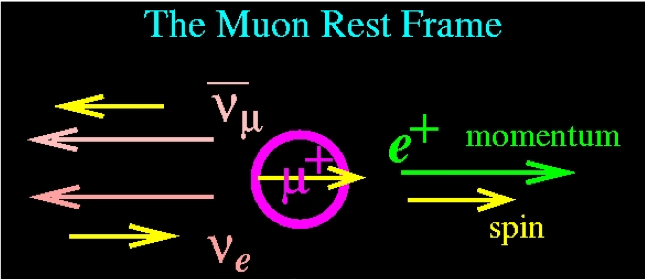
\includegraphics[width=0.9\textwidth]{MuonDecay}
	\label{fig:MuonDecay}
\end{figure}



-explain the physics
-explain how we get at the physics with our ring and detectors
-parity violation
-actually write out the decay states before explaining some things - well shouldn't these have been talked about before?? maybe not
-decay probabilities and all that
-don't measure all decay positrons
-By injecting a large ensemble of muons and 
-by measuring a subset of ensemble of muons....
-Careful with spin vs polarization





\begin{figure}[]
    \caption[ring]{clean up and possibly replace}   
    \centering
    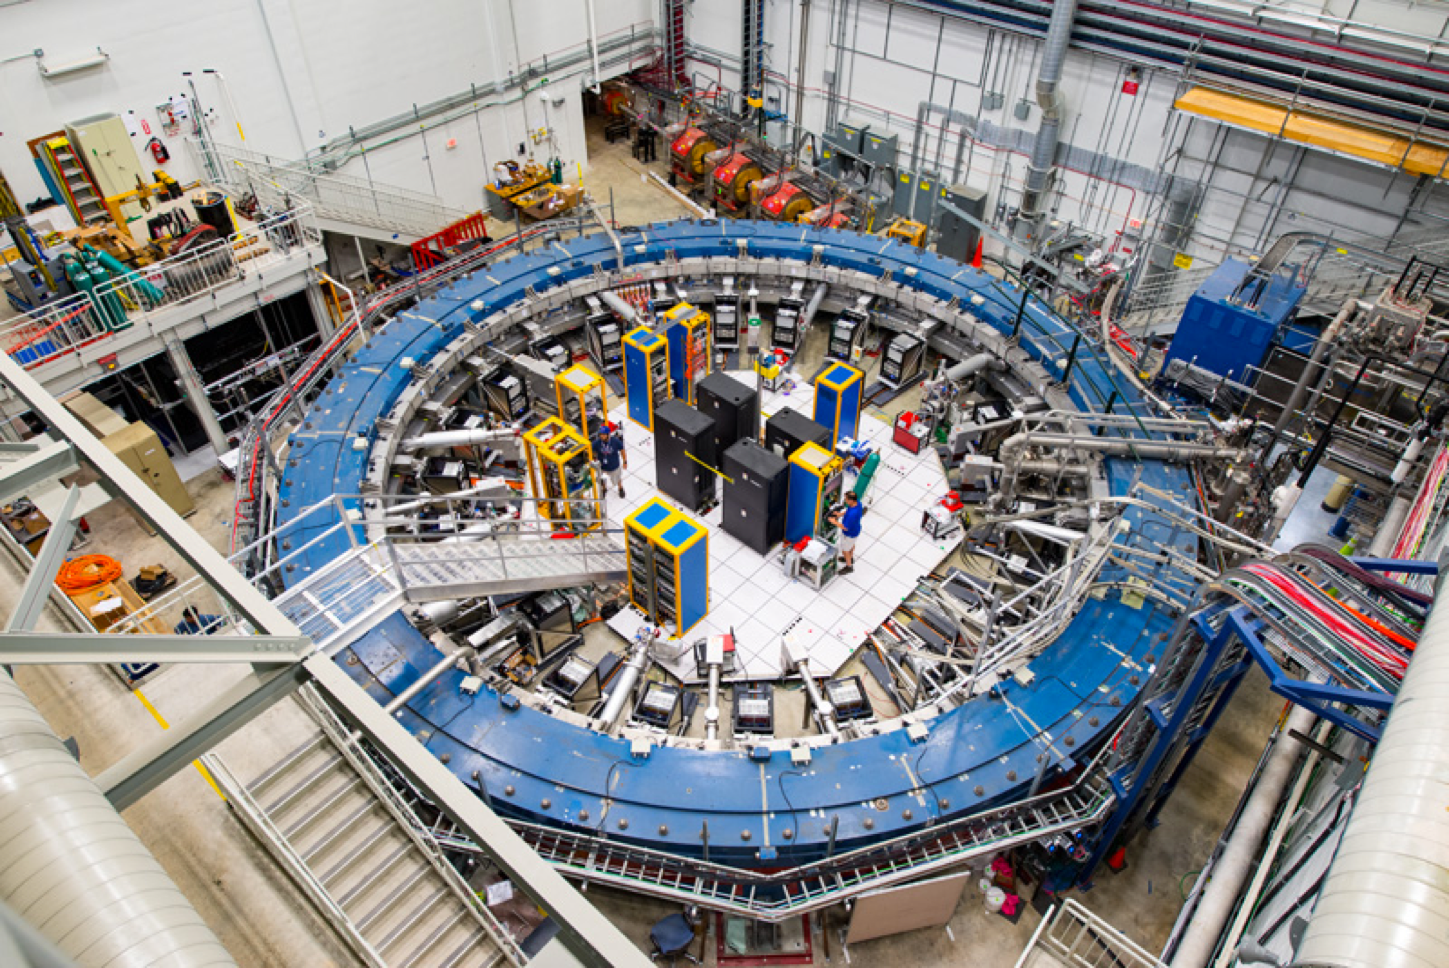
\includegraphics[width=0.9\textwidth]{ring}
    \label{fig:ring}
\end{figure}


\section{Accelerator}
\label{sec:Accelerator}


\cite{Stratakis:2017uci}


\section{Detector Systems}
\label{sec:DetectorSystems}

\begin{figure}[]
    \caption[TrackerCaloWithLines]{clean up and possibly replace}   
    \centering
    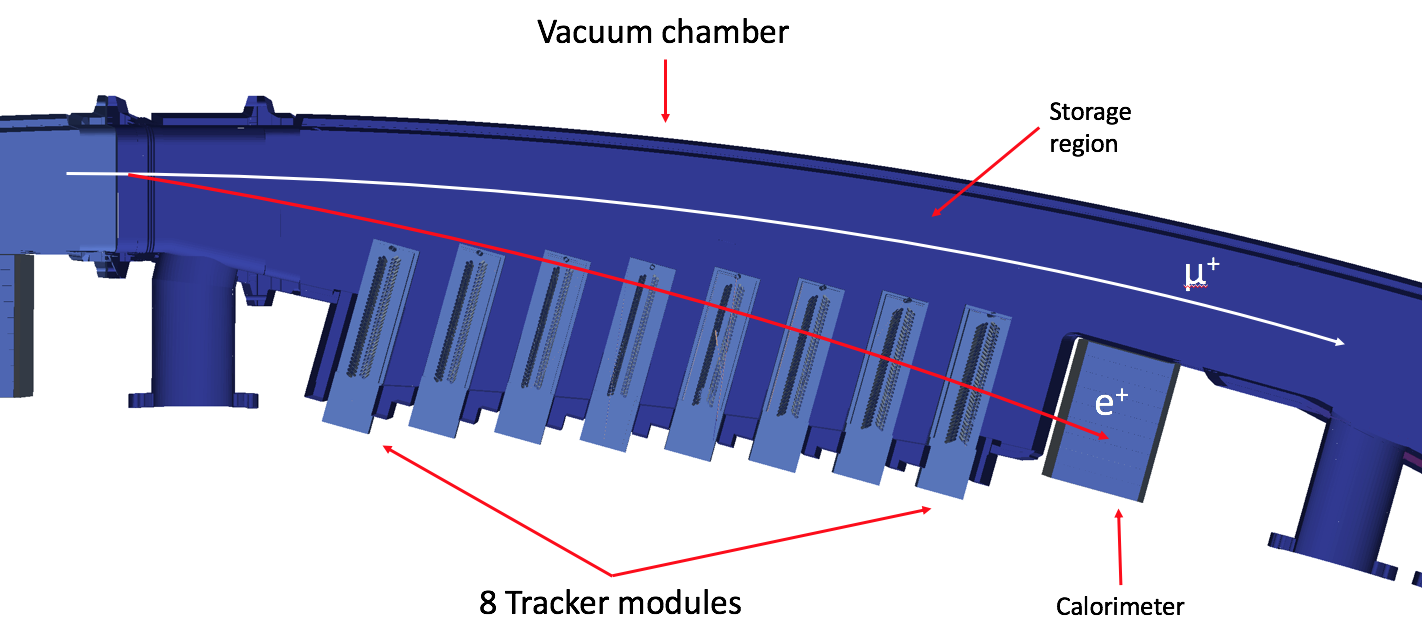
\includegraphics[width=0.9\textwidth]{TrackerCaloWithLines}
    \label{fig:TrackerCaloWithLines}
\end{figure}


\subsection{Calorimeters}
\label{sec:Calorimeters}

% what they do
% what they are
% how they work


Electromagnetic calorimeters measure the times and energies of decay positrons as they curl inward from the storage region. There are 24 calorimeters located symmetrically around the inside of the ring in close proximity to the vacuum chamber, as shown in Figure \ref{fig:}. They lie close to the storage region in order to measure a large fraction of the total number of observable decay positrons, including the high energy decay positrons which curl inward only slightly more than the muons themselves do. Because they are in close proximity to the storage region and by extension the magnetic field, the calorimeters must be non-magnetic in order to avoid perturbing the magnetic field. Each calorimeter consists of 54 channels of PbF\textsubscript{2} crystals arrayed in a 6 high by 9 wide array, which measure Cerenkov light emitted by the impinging positrons as they pass through the crystals \cite{Fienberg:2014kka}. (Picture of single calo and its crystals here.) Each crystal is 2.5 x 2.5 x 14 cm\textsuperscript{3}. The light is read out by large area silicon photo-multiplier (SiPM) sensors.


In order to determine \amu to the precision goal, there are modest requirements on the performance of the calorimeters. They must have a relative energy resolution of better than 5\% at 2 GeV, in order for proper event selection \cite{TDR}. They must have a timing resolution of better than 100 ps. The calorimeters must be able to resolve multiple incoming hits through temporal or spatial separation at 100\% efficiency for time separations of greater than 5 ns in order to reduce the pileup systematic error due to the high rate. Finally, the gain of the measured hits must be stable to $<$ 0.1\% over a 200 $\mu$s time period within a fill, and unaffected by a pulse arriving in the same channel a few nanoseconds earlier. The long term gain stability over a time period of order seconds must be $<$ 1\%.

(I've condensed quite a bit this section from the TDR - is that okay?)


To satisy these requirements SiPM sensors were chosen over PMTS...



and is wrapped in black Tedlar\textregistered\ foil



\cite{Kaspar:2016ofv} % second calo paper I need to cite



\subsection{Laser System}
\label{LaserSystem}
% should make this it's own section

For the gain, there is a laser system...

% make sure these are ordered properly
\cite{Anastasi:2015ssy}
\cite{Anastasi:2016luh}
\cite{Anastasi:2017sos}



% magnetic nature of calorimeters

% energy resolution
% gain
% high rate
% acceptance

% design of the vacuum chambers in order to...

% picture of calo placement
% picture of actual calo station




\subsection{Template Fitting}
\label{sec:TemplateFitting}





\subsection{Straw Trackers}
\label{sec:StrawTrackers}

The Muon \gmtwo Experiment at Fermilab uses straw tracking detectors to measure decay positron trajectories for the purpose of determining the muon beam distribution and its characteristics (and other things....). By fitting these tracks and extrapolating back to the average decay point, the beam can be characterized in a non-destructive fashion. See section blah. This is important because of the need for matching the average observed magnetic field of the decaying muons and their resulting decay positron directions which result in the \wa frequency.

The trackers are also useful for determining general beam diagnostics as well as the pitch correction and to a lesser extent the electric field correction (careful here). Cross-checking separately for pileup removal, hit verification, etc. is a powerful tool. Combining them in order to provide the muon distribution that the calorimeters directly see for the \wa calculation is perhaps the most important role of the tracker. With three trackers, approximately 5\% of decaying muons will result in measureable positron tracks assuming no pileup in the tracker, many of which do not hit the nearest calorimeter.

Each tracker module consists of 4 layers of 32 straws with a stereo angle of 7.5 degrees, the first two ``U'' layers oriented with the tops of the straws at a greater radial position, and the second two ``V'' layers oriented with the bottoms of the straws at a greater radial position. A tracking module is shown in Figure \ref{fig:tracker}. There are 2 tracker stations located in front of calorimeters 13 and 19, or at approximately 180 and 270 degrees counting clockwise from the top most point of the ring where the inflector resides. Figure \ref{fig:WorldCoordSys} shows this. (A third station sits empty after the inflector.) Each station consists of 8 tracking modules arranged in a staircase pattern that follows the curvature of the ring as seen in Figure \ref{fig:staircase}.

\begin{figure}[]
    \caption[Tracker module]{Shown is a picture of one of the many tracking modules used in the Muon \gmtwo experiment. The first layer of straws with a stereo angle of 7.5 degrees can be seen, with the other 3 straw layers hiding behind it. The beam direction is roughly into the page in this picture, to the left of the end of the module, and this view is what the decay positrons will see.}
    \centering
    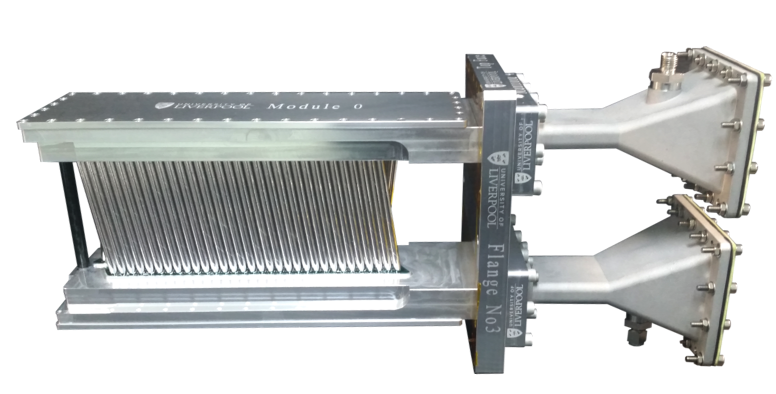
\includegraphics[width=0.9\textwidth]{Tracker}
    \label{fig:tracker}
\end{figure}

\begin{figure}[]
    \caption[Tracker module arrangement]{Tracker modules are arranged in the shown staircase pattern. In green and dark blue is the edge of the vacuum chamber (where the dark blue identifies the modification that was made to the old vacuum chambers), and it can be seen that vacuum chamber walls lie at the ends of the outside tracking modules. The position of a calorimeter can be seen in cyan at the right. The dark red spots are the locations of the outside magnet pole tips. From the shown geometry one can see that many positrons will hit either the tracker or the calorimeter but not both due to the acceptance differences.}
    \centering
    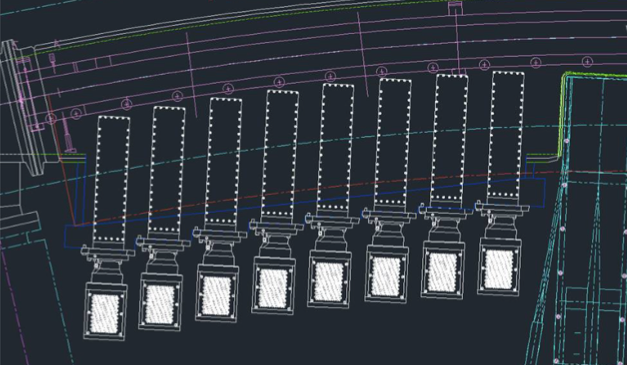
\includegraphics[width=0.9\textwidth]{trackerStation}
    \label{fig:staircase}
\end{figure}

In order to reduce the amount of multiple scattering within the straw tracking chambers as particles pass through them, the material of the straw trackers is minimized. Each straw is made of mylar foil, within which a 25 $\mu$m radius tungsten wire resides, and is filled with Argon-Ethane gas \cite{something}. Fast moving particles ionize the gas as they pass through it, and the resulting ions are drawn to the wire which is held at high voltage. When they reach the wire (and the mylar) a signal can be read out which tells us that a particle was seen to pass through the straw. By combining many such signals in a brief time span, we are able to construct tracks of incidient particles. (See section blah.) The resolution of hits within the straws is approximately 150 $\mu$m \cite{something}.

The signals of the straws are read out through...


